\hypertarget{prompting}{\section{Adaptation via prompting}}
\label{sec:prompting}

\begin{figure}
\centering
  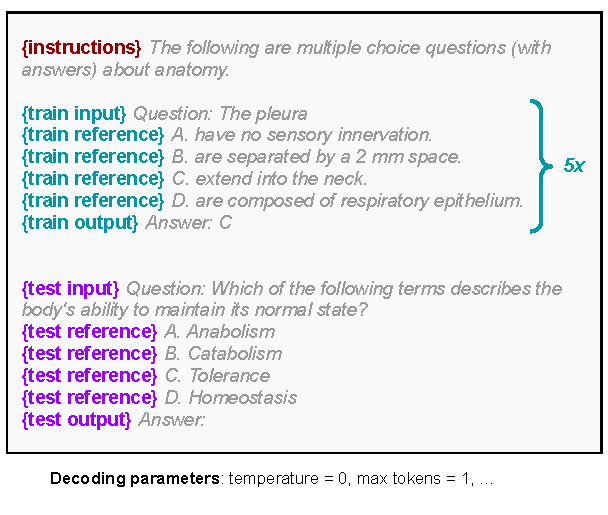
\includegraphics[width=0.5\textwidth]{figures/adaptation_v2.pdf}
  \caption{\textbf{Prompt formatting.} An example of how we structure and format the prompt for querying the language model.}
  \label{fig:adaptation-prompting}
\end{figure}

\begin{table*}[t]
\scriptsize
\centering
\begin{tabular}{clccc}
\toprule
& Parameter & Language Modeling & \truthfulqa & \cnndm \\
\midrule
\multirow{6}{*}{\shortstack{Prompt format\\ \refsec{prompting-test} \\\refsec{prompting-remainder}}} & Instructions & None & None & Summarize the given documents. \\
& Input prefix & None & Question:  & Document:  \\
& Reference prefix & None & None & None \\
& Output prefix & None & Answer: & Summary: \texttt{\{}\\ 
& Instance prefix & None & None & None \\
& Max training instances & 0 & \numincontext & \numincontext \\
\midrule 
\multirow{4}{*}{\shortstack{Decoding parameters\\ \refsec{decoding-parameters}}} & Temperature & 0 & 0 & 0.3  \\
& Max tokens & 0 & 5 & 128  \\
& Stop sequence(s) & None & \texttt{\textbackslash n} & \texttt{\}} \\
& Num. outputs & 0 & 1 & 1 \\
\midrule 
\multirow{2}{*}{\shortstack{Evaluation parameters }} & Num. runs & \numruns & \numruns & \numruns \\
& Max evaluation instances & \numevalinstances & \numevalinstances & \numevalinstances \\
\bottomrule
\end{tabular}
\caption{\textbf{Adaptation parameters.}
Example of the adaptation parameters specified for (i) language modeling scenarios, (ii) the \truthfulqa~question answering scenario, and (iii) the \cnndm~summarization scenario. 
We also include additional parameters required to fully specify evaluation (\ie the number of evaluation instances and runs, which influence the statistical validity and reliability of the results), though they are not strictly part of the adaptation process.}
\label{tab:adaptation-decisions}
\end{table*}

Adaptation transforms a raw language model into a system that makes predictions on test instances.
In short, we use prompting as our adaptation method with \numincontext in-context examples (when in-context examples are included) as depicted in \reffig{adaptation-prompting}.
However, many lower-level details must be specified to fully define the adaptation procedure: we discuss important conceptual details here and defer the remainder to \refapp{adaptation}.
\reftab{adaptation-decisions} provides example scenarios along with the full set of adaptation parameters.

\paragraph{In-context examples.}
Since we include \numincontext in-context examples, two core decisions are why we use this number of examples and how we select the examples.
We follow \citet{brown2020gpt3} in their choice of the number, testing in \refsec{prompting-analysis} how the number of examples influences performance. 
To select examples, we sample examples to ensure class coverage (for classification coverage) in order of class frequency, so the \numincontext most frequent classes will be represented in-context.
Critically, we choose to fix the in-context examples across all evaluation instances, in contrast to prior work \citep[\eg][]{brown2020gpt3}, to more accurately perform few-shot evaluation \citep{perez2021true}.
While more realistic, this also implies our model performance can be more sensitive to the random choice of in-context examples.
Therefore, we re-run all experiments \numruns times, only varying the randomness in in-context sample selection, to estimate this variance: in \refsec{prompting-analysis}, we show results can be especially high variance for some scenarios.

\paragraph{Prompt formatting.}
Beyond the in-context examples and evaluation instance, there are many other mechanistic nuances involved in formatting the exact string that submitted to the language model.
Prior work has extensively shown that the design of prompts matters \citep{lescao2021prompt, liu2022incontext}, with \citet{bach2022promptsource} introducing a repository for prompts.\footnote{\url{https://github.com/bigscience-workshop/promptsource}}
Since we more broadly view language models as \textit{interfaces}, we treat prompts as user behavior rather than explicitly optimizing prompts \citep{shin2020autoprompt, zhou2022large}.
Moving forward, we further expect that it may be desirable for language models to be \textit{interoperable} meaning different models should be standardized such that they all work well for similar user prompting behavior.
We provide initial evidence of how model performance varies in the exact string formatting of the inputs in \refsec{prompting-analysis}.

\paragraph{Adaptation strategy.}
For many scenarios (\eg language modeling, text summarization), the way to interact with a language model may appear clear. 
However, in the case of multiple choice classification, each instance has several answer choices as references (usually with one marked as correct).
This structure affords flexibility in how to use a language model that traditionally does not exist in classification (where a model necessarily predicts a distribution over answer choices with the prediction being the argmax).

Prior work introduces two classes of approaches to address adaptation for multiple choice scenarios.
The first is the \textit{separate} approach employed by \citet{brown2020gpt3}, where each choice is independently scored by concatenating it with the question and computing its probability according to the LM.
In this approach, the probabilities may be further \textit{calibrated} by the probability the LM assigns to the answer choice alone.
The second is the \textit{joint} approach employed by \citet{hendrycks2021measuring}, where all the choices are concatenated with the question to form a prompt (e.g., ``\texttt{<question> A.\,<choice\,1> B.\,<choice\,2>  Answer:}'') and the LM predicts the choice index (e.g., \texttt{A} or \texttt{B}).
This resembles how one might see a multiple choice question presented on an exam or test.
In \refsec{prompting-analysis}, we vary this adaptation strategy to test the influence on performance: we find the strategy significantly influences accuracy (among other metrics), and the most accurate strategy depends on the scenario (\ie no strategy is uniformly more accurate). 